%        File: prac1.tex
%     Created: Sat Feb 09 01:00  2019 S
% Last Change: Sat Feb 09 01:00  2019 S
%
\documentclass[a4paper, 12pt]{article}
\usepackage[]{amsmath}
\usepackage{amssymb}
\usepackage{float}
\usepackage[]{graphicx}

\title{Control Systems 4A Practical 1 Report}
\author{Ruan de Bruyn, 216054484 \and Quintin Kruger, VERANDER HIERDIE}

\begin{document}

\pagenumbering{gobble}
\begin{titlepage}
  \maketitle
\end{titlepage}

\pagenumbering{roman}
\tableofcontents
\newpage
\pagenumbering{arabic}

\section{Transfer Function}
	As a quick summary of the theory given in the practical assignment, the
	equation that governs this system, is given by

	\begin{equation}
	  \frac{d^2}{dt^2} x = -\frac{5g}{7} \sin(\theta)
	  \label{eq:system_complete}
	\end{equation}

	If we make the assumption for this system that the angle $\theta$ is small,
	then we can use small-angle approximation to say that $\sin \theta \approx
	\theta$, and thus \eqref{eq:system_complete} becomes

	\begin{equation}
	  \frac{d^2}{dt^2} x = -\frac{5g}{7} \theta
	  \label{eq:system_simplified}
	\end{equation}

	From here, we can a Laplace transform to calculate the transfer function of
	our system, using \eqref{eq:system_simplified}:

	\begin{equation*}
	  \begin{array}{rcl}
		\mathcal{L}\left[ \frac{d^2}{dt^2}x \right] & = & \mathcal{L}\left[ -\frac{5g}{7}\theta \right] \\
		s^2 X(s) & = & -\frac{5g}{7}\Theta(s) \\
		\frac{X(s)}{\Theta(s)}  & = & -\frac{5g}{7s^2} \\
	  \end{array}
	  \label{eq:transfer_function}
	\end{equation*}
	
	Taking the constant $g = 9.8 \, m \cdot s^{-2}$, this leaves us with a final transfer function of

	\begin{equation}
	  T(s) = -\frac{5g}{7s^2} = -\frac{7}{s^2}
	  \label{eq:tf_final}
	\end{equation}

% endsection Transfer Function

\section{Implementation and Analysis}
	The Octave code that was used to design the PID controller in the rest of
	this report are given below\\\\\noindent
	\texttt{function plotsys(Kp, Ki, Kd)\\\noindent
  ts = - 5 * 9.8 / (7 * tf('s'));\\\noindent
  sys = feedback(ts * pid(Kp, Ki, Kd))\\\noindent
  step(sys);\\\noindent
endfunction}

This function simply obtains the transfer function obtained in
\eqref{eq:tf_final}, finds the equivalent function of the plant and controller
with the specified constants in a negative feedback loop, and then graphs the
output response. The design strategy of the PID controller for our system is to
have a fairly quick rise time, but also with very little overshoot. A quick
rise time is necessary, because if our system is too slow to react, the ball
may fall off of one of the ends of the beam. Overshoot should be kept as low as
possible as well, because a large overshoot could very well result in the ball
falling off the beam too, especially if the commanding signal desires the
location of the ball to be near one of the edges of the beam.

From theory, we would hypothesize that we should have a large $K_p$ and $K_d$,
as a large $K_p$ would result in a quick rise time and a large $K_d$ would
prevent large amounts of overshoot. $K_i$, then, should be the variable to keep
small in relation to $K_p$ and $K_d$, as $K_i$ contributes to a quick rise
time, but also to overshoot. With this in mind, we choose our variables as
follows:

\begin{equation}
  \begin{array}{rcl}
	K_p & = & 70 \\
	K_i & = & 18 \\
	K_d & = & 40
  \end{array}
  \label{eq:pid_constants}
\end{equation}

The response given by this system of constants is

\begin{figure}[H]
	\centering
	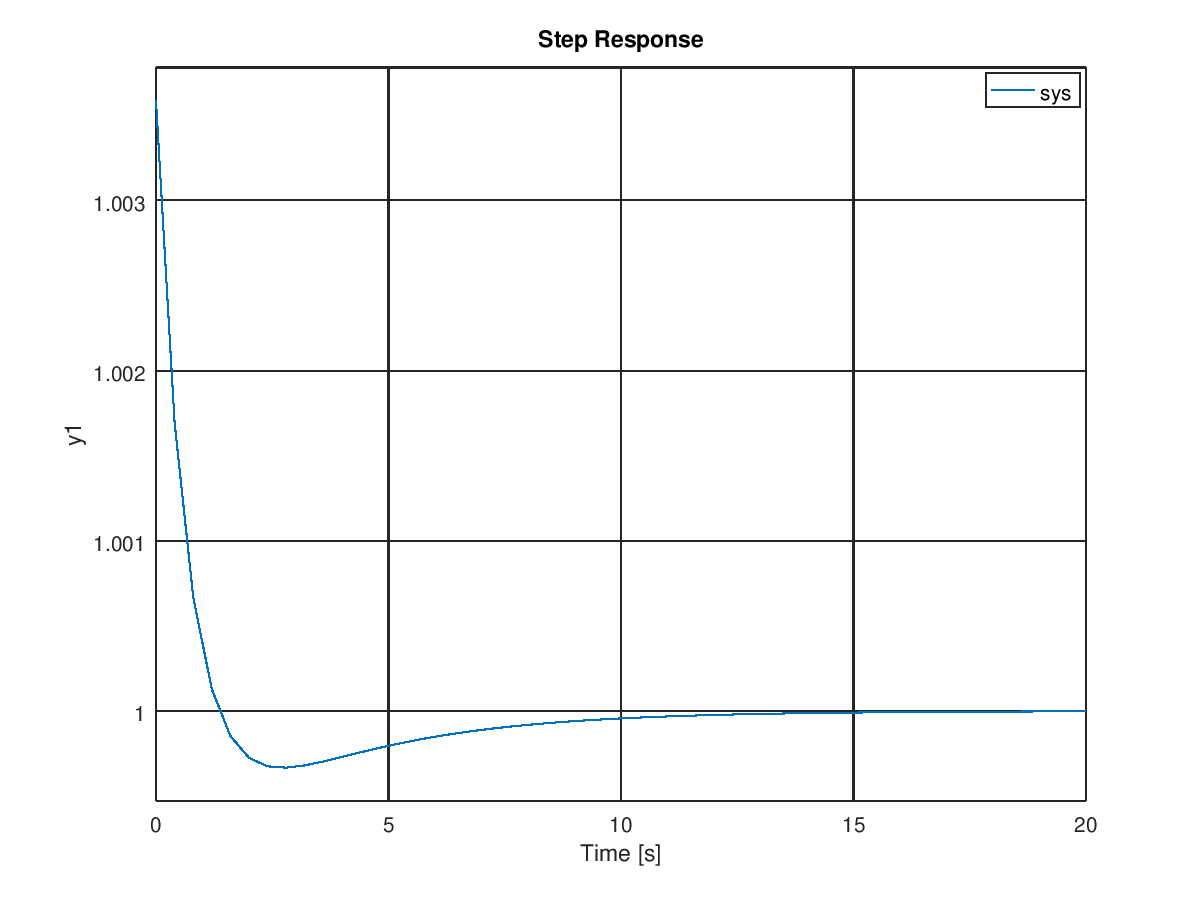
\includegraphics[width=\textwidth]{response.png}
	\caption{System response with constants chosen in \eqref{eq:pid_constants}}
	\label{fig:response}
\end{figure}

If we decide to let the rise time for this system be defined as the time it
takes the response to reach 0.1\% of it's final value, then the rise time $t_r
= 0.67s$. The overshoot is 0.9997, which means that $\%OS = 0.03$. Finally, if
we take the settling time to be the time it takes the transfer function to
reach 0.0001 of its final value, then we have $t_s = 7.33s$. The final values
are then summarised below as

\begin{equation}
  \begin{array}{rcl}
    t_r & = & 0.67 \\
    t_s & = & 7.33 \\
    \%OS & = & 0.03 \\
  \end{array}
  \label{eq:finalstats}
\end{equation}

% endsecion Implementation and Analysis
\end{document}
